% Options for packages loaded elsewhere
\PassOptionsToPackage{unicode}{hyperref}
\PassOptionsToPackage{hyphens}{url}
\PassOptionsToPackage{dvipsnames,svgnames,x11names}{xcolor}
\documentclass[
  11pt,
]{article}
\usepackage{xcolor}
\usepackage[margin=0.5in]{geometry}
\usepackage{amsmath,amssymb}
\setcounter{secnumdepth}{5}
\usepackage{iftex}
\ifPDFTeX
  \usepackage[T1]{fontenc}
  \usepackage[utf8]{inputenc}
  \usepackage{textcomp} % provide euro and other symbols
\else % if luatex or xetex
  \usepackage{unicode-math} % this also loads fontspec
  \defaultfontfeatures{Scale=MatchLowercase}
  \defaultfontfeatures[\rmfamily]{Ligatures=TeX,Scale=1}
\fi
\usepackage{lmodern}
\ifPDFTeX\else
  % xetex/luatex font selection
  \setmainfont[]{Helvetica}
  \setmonofont[]{Menlo}
\fi
% Use upquote if available, for straight quotes in verbatim environments
\IfFileExists{upquote.sty}{\usepackage{upquote}}{}
\IfFileExists{microtype.sty}{% use microtype if available
  \usepackage[]{microtype}
  \UseMicrotypeSet[protrusion]{basicmath} % disable protrusion for tt fonts
}{}
\makeatletter
\@ifundefined{KOMAClassName}{% if non-KOMA class
  \IfFileExists{parskip.sty}{%
    \usepackage{parskip}
  }{% else
    \setlength{\parindent}{0pt}
    \setlength{\parskip}{6pt plus 2pt minus 1pt}}
}{% if KOMA class
  \KOMAoptions{parskip=half}}
\makeatother
\usepackage{longtable,booktabs,array}
\newcounter{none} % for unnumbered tables
\usepackage{calc} % for calculating minipage widths
% Correct order of tables after \paragraph or \subparagraph
\usepackage{etoolbox}
\makeatletter
\patchcmd\longtable{\par}{\if@noskipsec\mbox{}\fi\par}{}{}
\makeatother
% Allow footnotes in longtable head/foot
\IfFileExists{footnotehyper.sty}{\usepackage{footnotehyper}}{\usepackage{footnote}}
\makesavenoteenv{longtable}
\usepackage{graphicx}
\makeatletter
\newsavebox\pandoc@box
\newcommand*\pandocbounded[1]{% scales image to fit in text height/width
  \sbox\pandoc@box{#1}%
  \Gscale@div\@tempa{\textheight}{\dimexpr\ht\pandoc@box+\dp\pandoc@box\relax}%
  \Gscale@div\@tempb{\linewidth}{\wd\pandoc@box}%
  \ifdim\@tempb\p@<\@tempa\p@\let\@tempa\@tempb\fi% select the smaller of both
  \ifdim\@tempa\p@<\p@\scalebox{\@tempa}{\usebox\pandoc@box}%
  \else\usebox{\pandoc@box}%
  \fi%
}
% Set default figure placement to htbp
\def\fps@figure{htbp}
\makeatother
\setlength{\emergencystretch}{3em} % prevent overfull lines
\providecommand{\tightlist}{%
  \setlength{\itemsep}{0pt}\setlength{\parskip}{0pt}}
\usepackage{fvextra}
\DefineVerbatimEnvironment{Highlighting}{Verbatim}{breaklines,breakanywhere,commandchars=\\\{\}}
\usepackage{graphicx}
\usepackage{float}
\usepackage{microtype}
\usepackage{setspace}
\setstretch{1.05}
\setlength{\emergencystretch}{1em}
\makeatletter
\def\maxwidth{\ifdim\Gin@nat@width>\linewidth\linewidth\else\Gin@nat@width\fi}
\def\maxheight{\ifdim\Gin@nat@height>0.85\textheight0.85\textheight\else\Gin@nat@height\fi}
\makeatother
\setkeys{Gin}{width=\maxwidth,height=\maxheight,keepaspectratio}
\floatplacement{figure}{H}
\usepackage{bookmark}
\IfFileExists{xurl.sty}{\usepackage{xurl}}{} % add URL line breaks if available
\urlstyle{same}
\hypersetup{
  pdftitle={Story 2: Can the FED Control Inflation and Maintain Full Employment (Last 25 Years)},
  pdfauthor={Randy Howk},
  colorlinks=true,
  linkcolor={blue},
  filecolor={Maroon},
  citecolor={Blue},
  urlcolor={blue},
  pdfcreator={LaTeX via pandoc}}

\title{Story 2: Can the FED Control Inflation and Maintain Full
Employment (Last 25 Years)}
\author{Randy Howk}
\date{2026-02-22}

\begin{document}
\maketitle

{
\setcounter{tocdepth}{2}
\tableofcontents
}
\section{Purpose and Research
Questions}\label{purpose-and-research-questions}

The Federal Reserve's dual mandate from Congress is to:

\begin{enumerate}
\def\labelenumi{\arabic{enumi}.}
\tightlist
\item
  Maintain \textbf{stable prices} (control inflation)\\
\item
  Maintain \textbf{maximum employment} (low unemployment)
\end{enumerate}

These objectives can conflict, especially around recessions and supply
shocks.

\textbf{Main Question:}\\
\textbf{Has the FED been able to fulfill the mandate given to it by
Congress over the last 25 years?}

This analysis is \textbf{observational} and focuses on time ordering and
consistency with known policy lags. It does \textbf{not} claim causal
proof.

\section{Story Development Focus}\label{story-development-focus}

\textbf{Focus Point:} \emph{Visual selection framework + slide messaging
technique}

\begin{itemize}
\tightlist
\item
  Use a small set of repeatable, consistent visuals (simplicity +
  uniformity)
\item
  Use clear benchmark lines and shaded ``episodes'' to emphasize ``good
  vs bad'' periods (saliency)
\item
  Use separate panels rather than dual axes to avoid distortion
  (fidelity + efficacy)
\item
  Use a lag-aware view to respect the timing relationship (Fed reacts to
  inflation; unemployment responds later)
\end{itemize}

\section{Data Sources (API)}\label{data-sources-api}

We pull monthly data for the last 25 years via API:

\begin{itemize}
\tightlist
\item
  \textbf{CPI-U (All items, SA)} --- BLS series: \texttt{CUSR0000SA0}\\
\item
  \textbf{Unemployment Rate} --- BLS series: \texttt{LNS14000000}\\
\item
  \textbf{Effective Federal Funds Rate} --- FRED series:
  \texttt{FEDFUNDS}
\end{itemize}

\begin{quote}
\textbf{API keys (recommended):}\\
- BLS v2 registration key: set \texttt{BLS\_KEY} in \texttt{.Renviron}\\
- FRED API key: set \texttt{FRED\_KEY} in \texttt{.Renviron}
\end{quote}

\begin{center}\rule{0.5\linewidth}{0.5pt}\end{center}

\section{Theory}\label{theory}

The core policy theory is that the Fed can move one tool, the policy
interest rate, to influence both sides of its mandate over time:

\begin{itemize}
\tightlist
\item
  Higher interest rates reduce borrowing, spending, and pricing
  pressure, helping inflation move down.
\item
  Lower interest rates support borrowing and demand, helping employment
  recover when labor markets weaken.
\end{itemize}

In practice, this is not instant. Inflation and unemployment usually
respond with lags, and shocks can temporarily break the tradeoff.

Band legend for theory visuals: - Light red band = inflation benchmark
margin-of-error around the dashed inflation target line. - Light blue
band = unemployment benchmark margin-of-error around the dashed
unemployment benchmark line.

\subsection{Theory Slide 1: Interest Rates and
Inflation}\label{theory-slide-1-interest-rates-and-inflation}

\pandocbounded{
\includegraphics[keepaspectratio]{Story2_updated_files/figure-latex/theory_slide_1-1.pdf}}

\subsection{Theory Slide 2: Interest Rates and
Unemployment}\label{theory-slide-2-interest-rates-and-unemployment}

\pandocbounded{
\includegraphics[keepaspectratio]{Story2_updated_files/figure-latex/theory_slide_2-1.pdf}}

\section{API Helpers}\label{api-helpers}

\section{Episodes to Highlight (Good vs Bad
Performance)}\label{episodes-to-highlight-good-vs-bad-performance}

These shaded windows act like ``chapters'' in the story.

\section{Pull and Prepare Data (Last 25
Years)}\label{pull-and-prepare-data-last-25-years}

\section{Visual Theme (Uniformity +
Simplicity)}\label{visual-theme-uniformity-simplicity}

\section{Visualization 1 --- Mandate Scorecard Timeline (No Dual
Axis)}\label{visualization-1-mandate-scorecard-timeline-no-dual-axis}

This stacks three aligned time series (inflation, unemployment, policy
rate).

\pandocbounded{
\includegraphics[keepaspectratio]{Story2_updated_files/figure-latex/viz_timeline-1.pdf}}

\pandocbounded{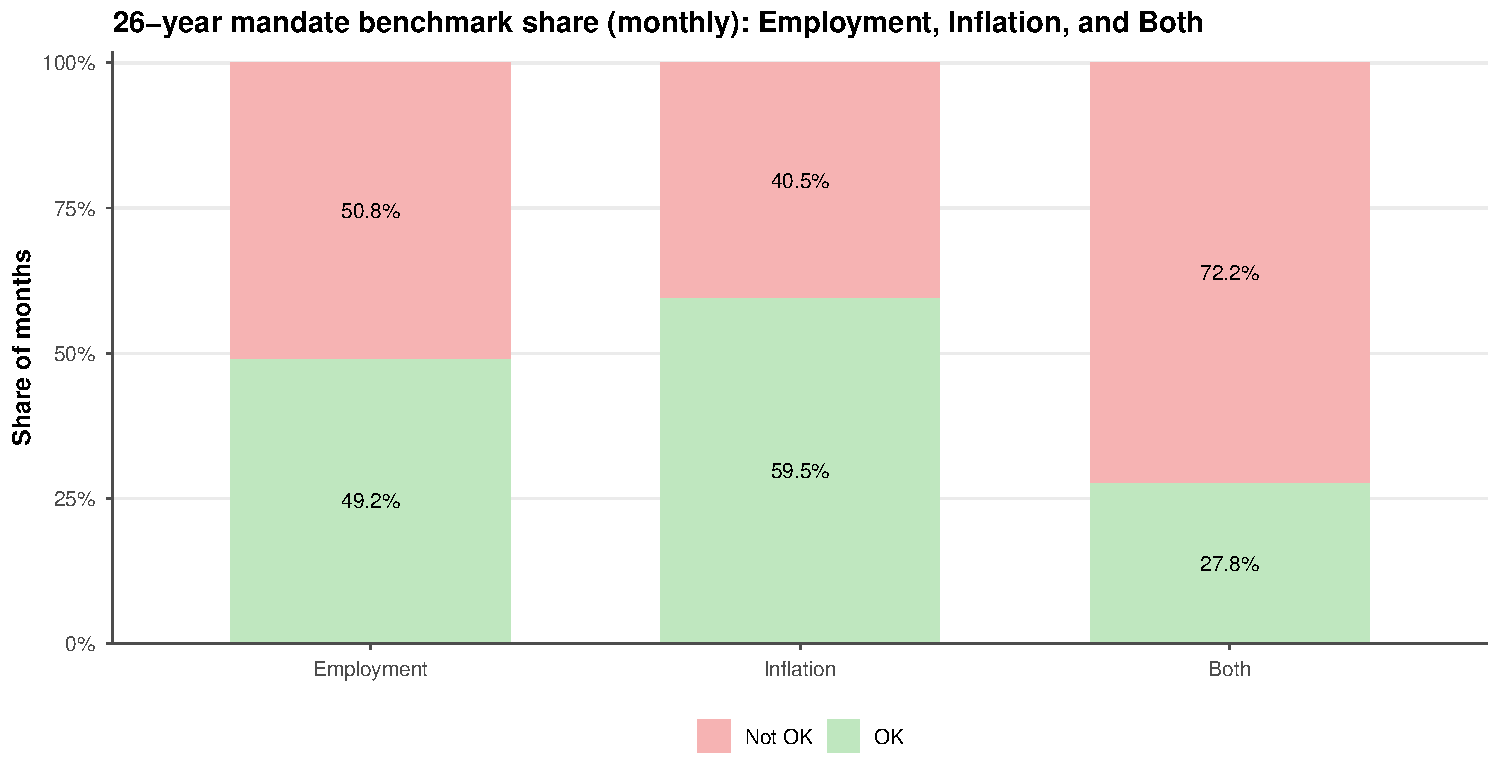
\includegraphics[keepaspectratio]{Story2_updated_files/figure-latex/viz_timeline_stacked_26y-1.pdf}}

\section{Period deep-dives (Theory-style
charts)}\label{period-deep-dives-theory-style-charts}

For each period of interest, we reproduce \textbf{two theory-style,
dual-axis line charts}:

\begin{enumerate}
\def\labelenumi{\arabic{enumi})}
\tightlist
\item
  \textbf{Fed Funds vs Unemployment} (dashed = unemployment, right
  axis)\\
\item
  \textbf{Fed Funds vs Inflation (CPI YoY)} (dashed = inflation, right
  axis)
\end{enumerate}

Each chart \textbf{rescales the right axis per-period} so the two lines
are visually comparable and the relationship is clear.

\subsection{Dot-com bust (2000-2003)}\label{dot-com-bust-2000-2003}

\pandocbounded{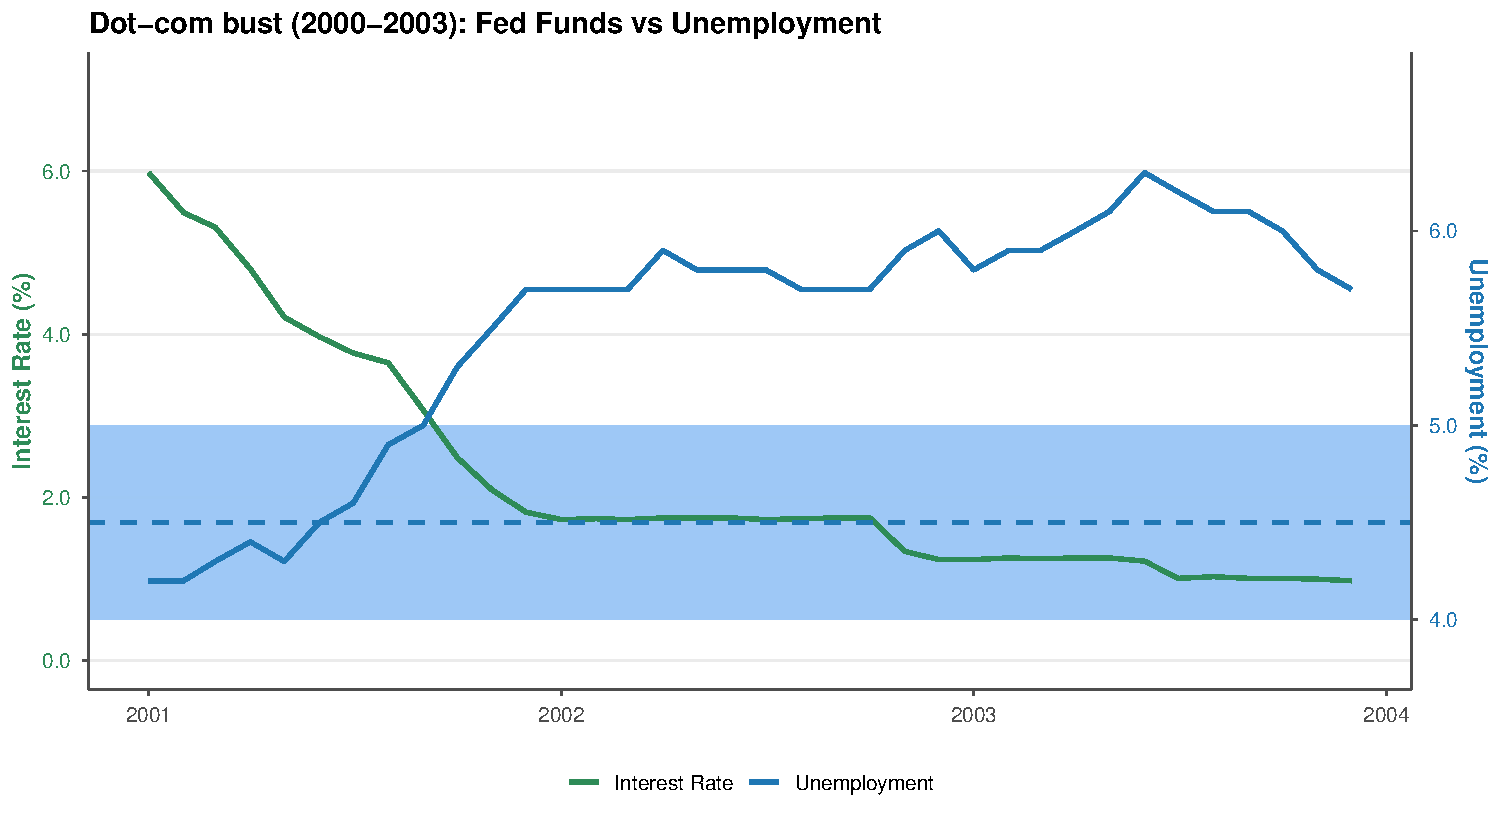
\includegraphics[keepaspectratio]{Story2_updated_files/figure-latex/31_dotcom_unemp-1.pdf}}

\pandocbounded{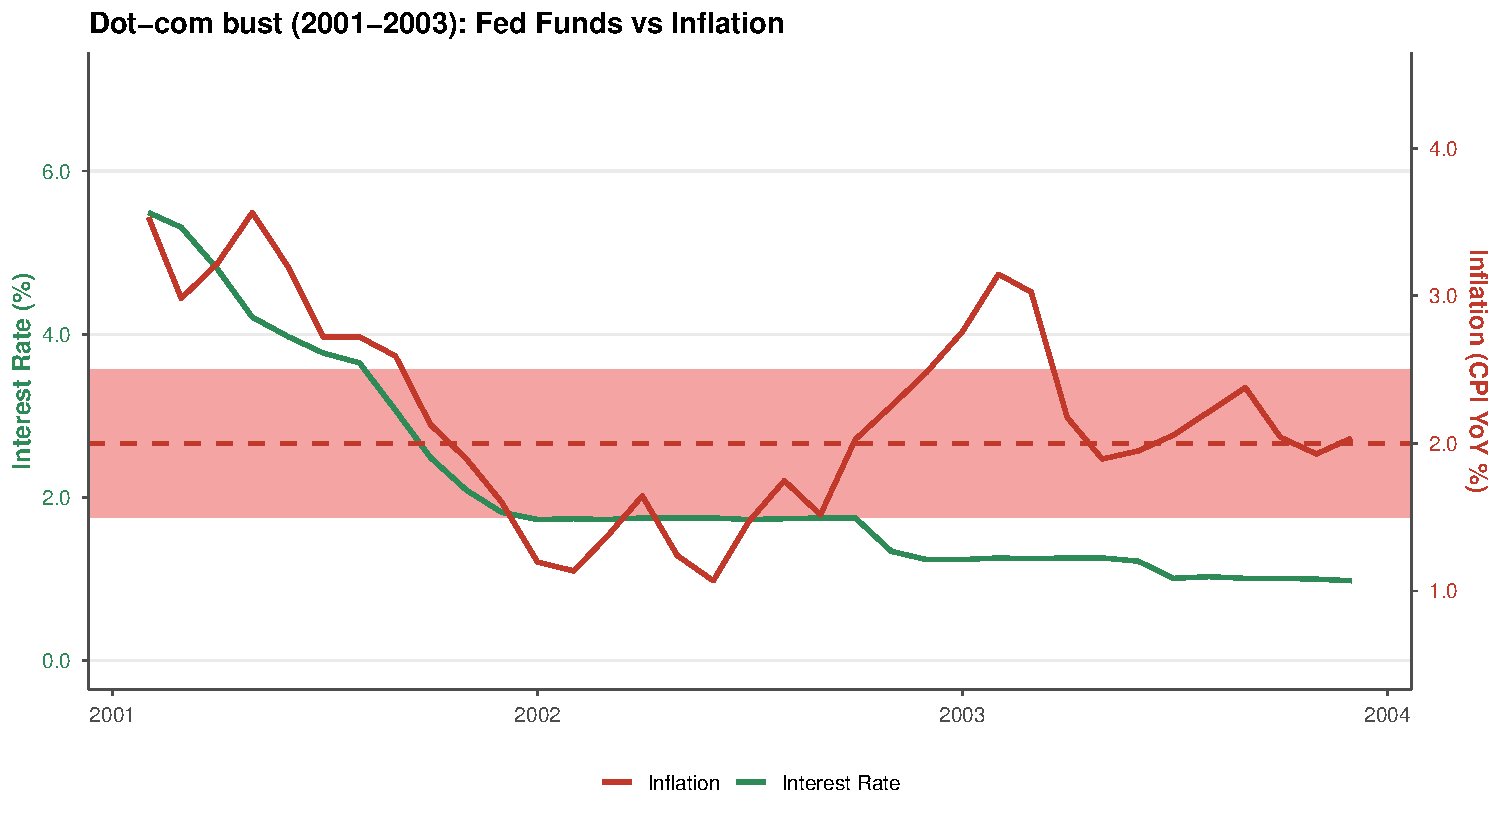
\includegraphics[keepaspectratio]{Story2_updated_files/figure-latex/32_dotcom_infl-1.pdf}}

\pandocbounded{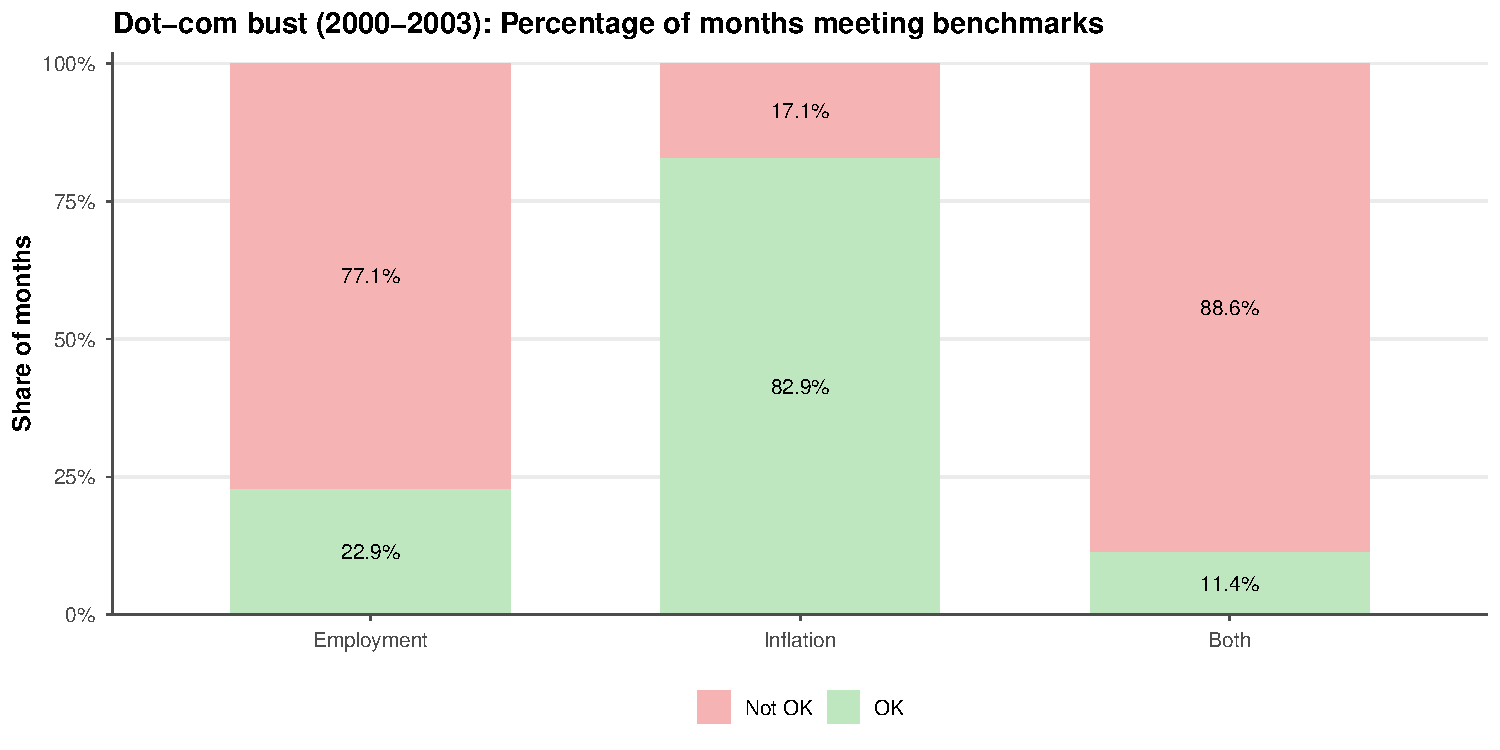
\includegraphics[keepaspectratio]{Story2_updated_files/figure-latex/32b_dotcom_stacked-1.pdf}}

\subsection{Financial crisis + aftermath
(2008-2012)}\label{financial-crisis-aftermath-2008-2012}

\pandocbounded{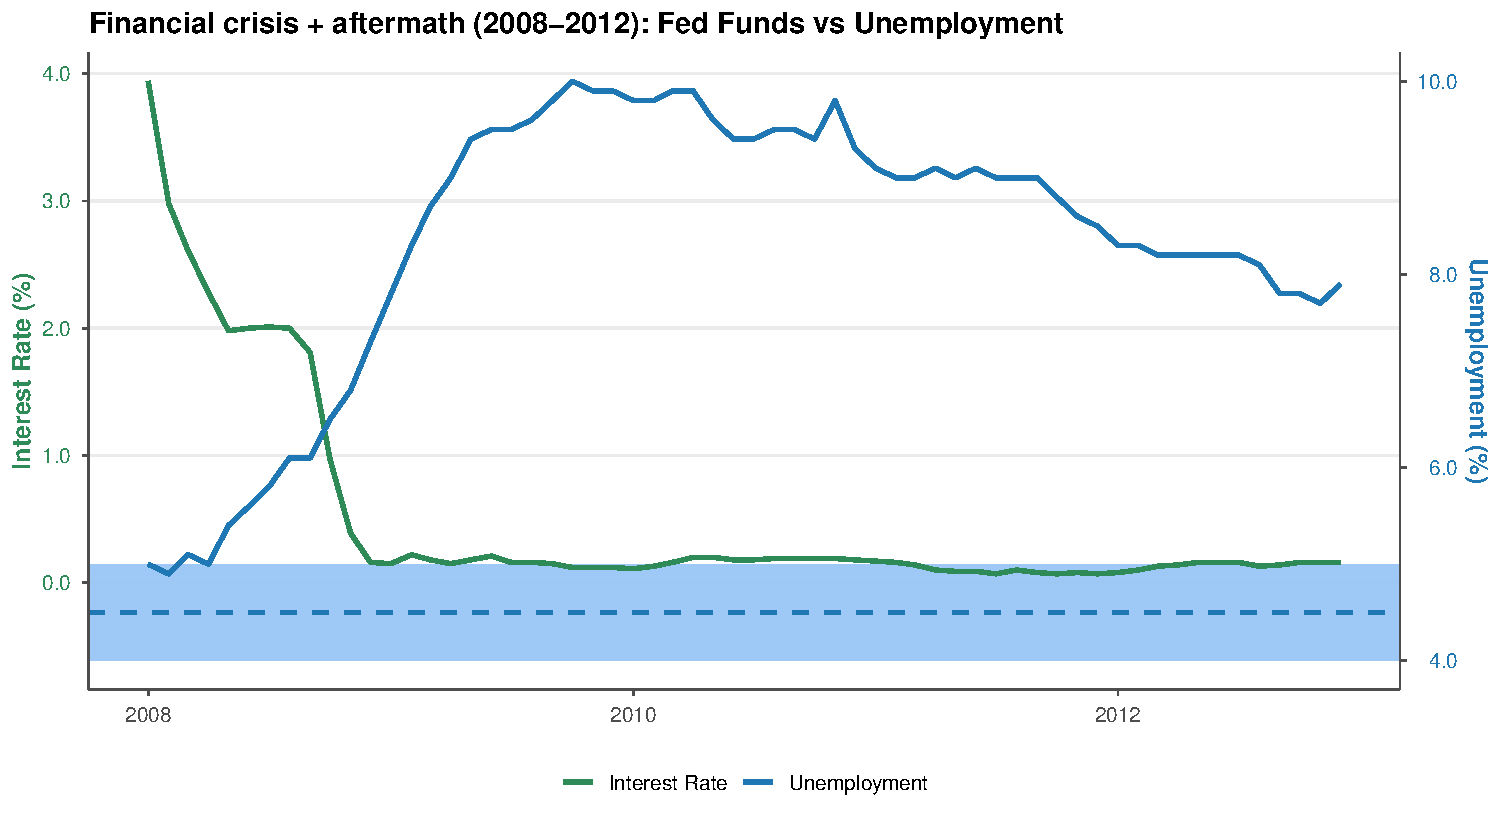
\includegraphics[keepaspectratio]{Story2_updated_files/figure-latex/41_gfc_unemp-1.pdf}}

\pandocbounded{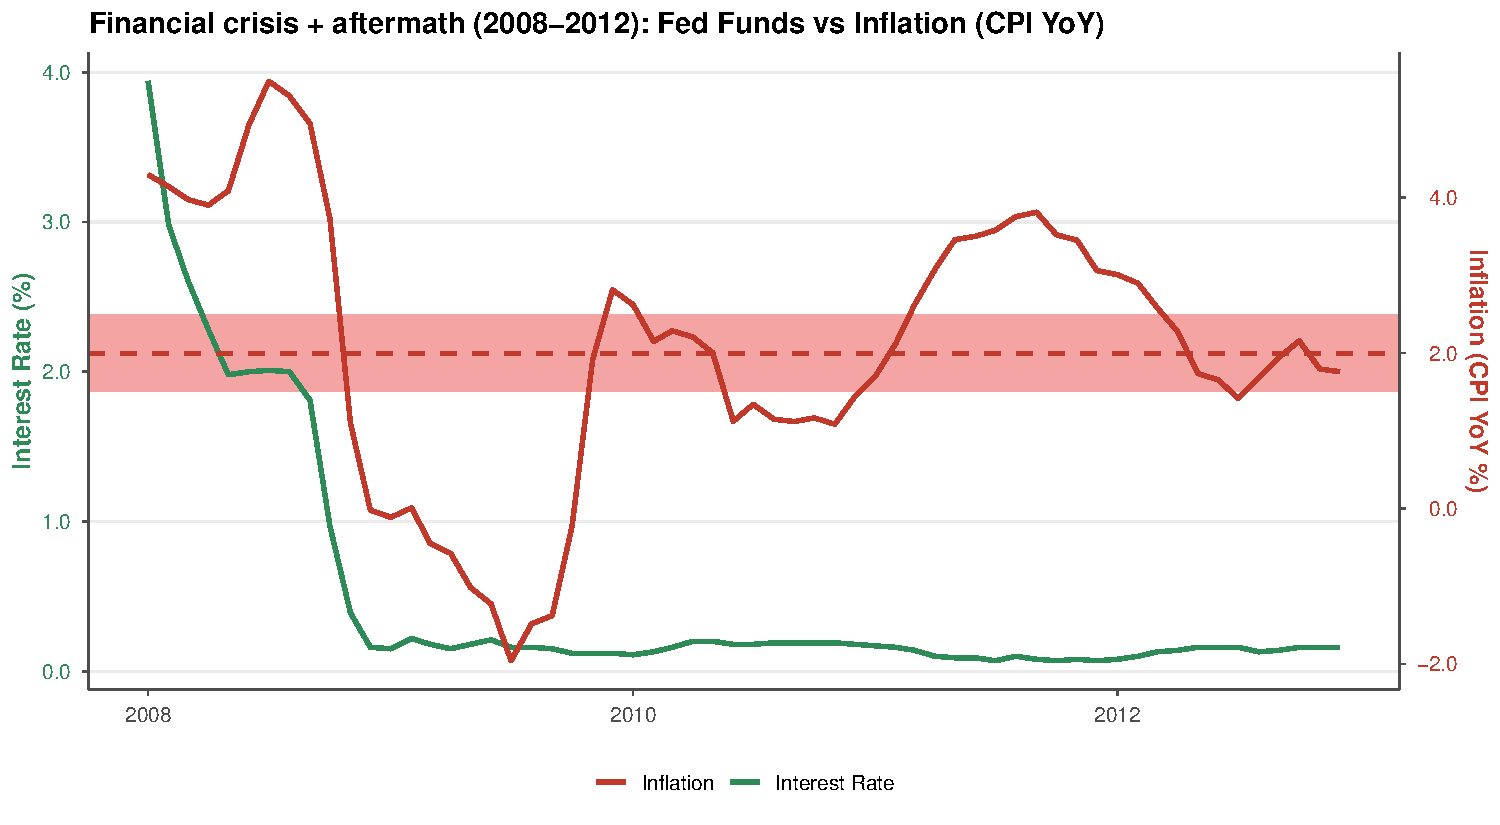
\includegraphics[keepaspectratio]{Story2_updated_files/figure-latex/42_gfc_infl-1.pdf}}

\pandocbounded{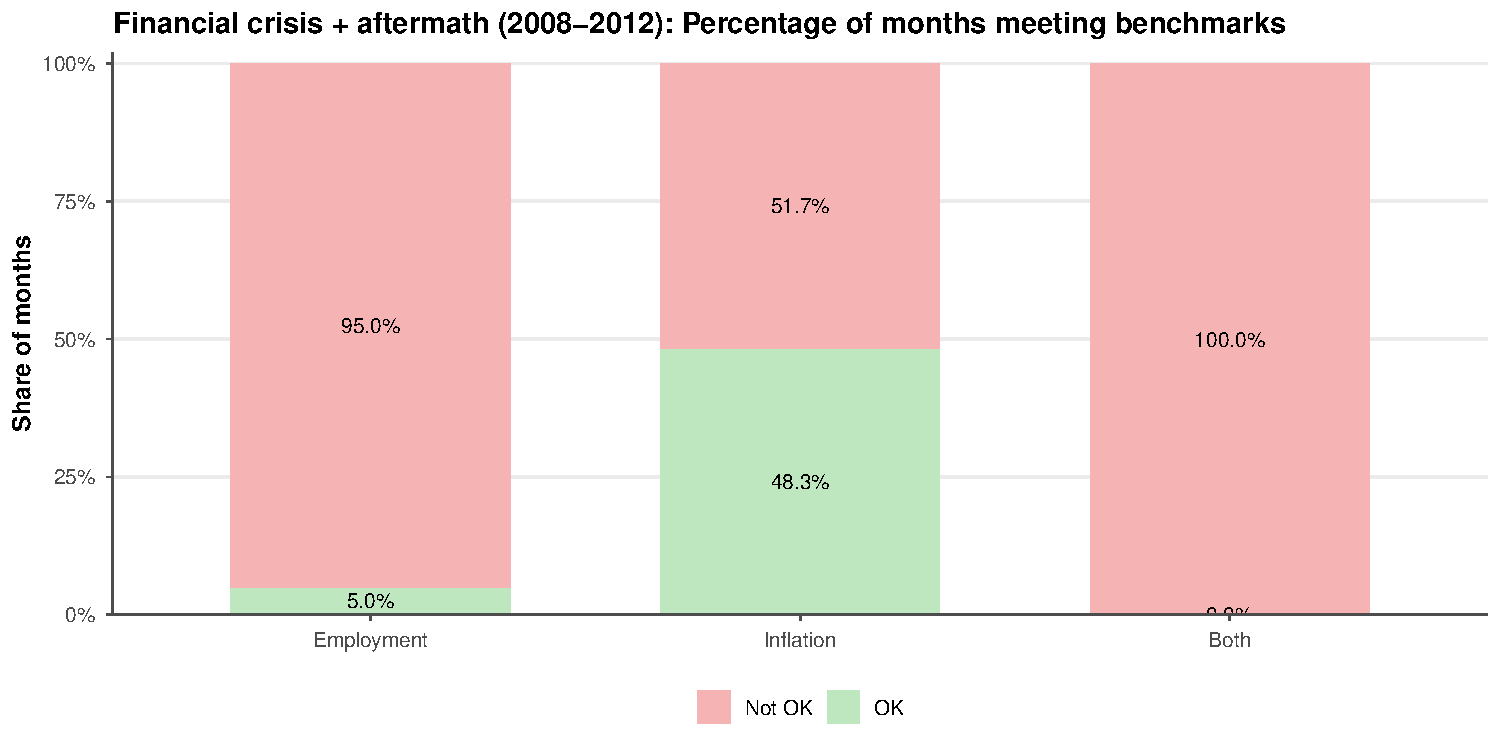
\includegraphics[keepaspectratio]{Story2_updated_files/figure-latex/42b_gfc_stacked-1.pdf}}

\subsection{COVID era (2020-2023)}\label{covid-era-2020-2023}

\pandocbounded{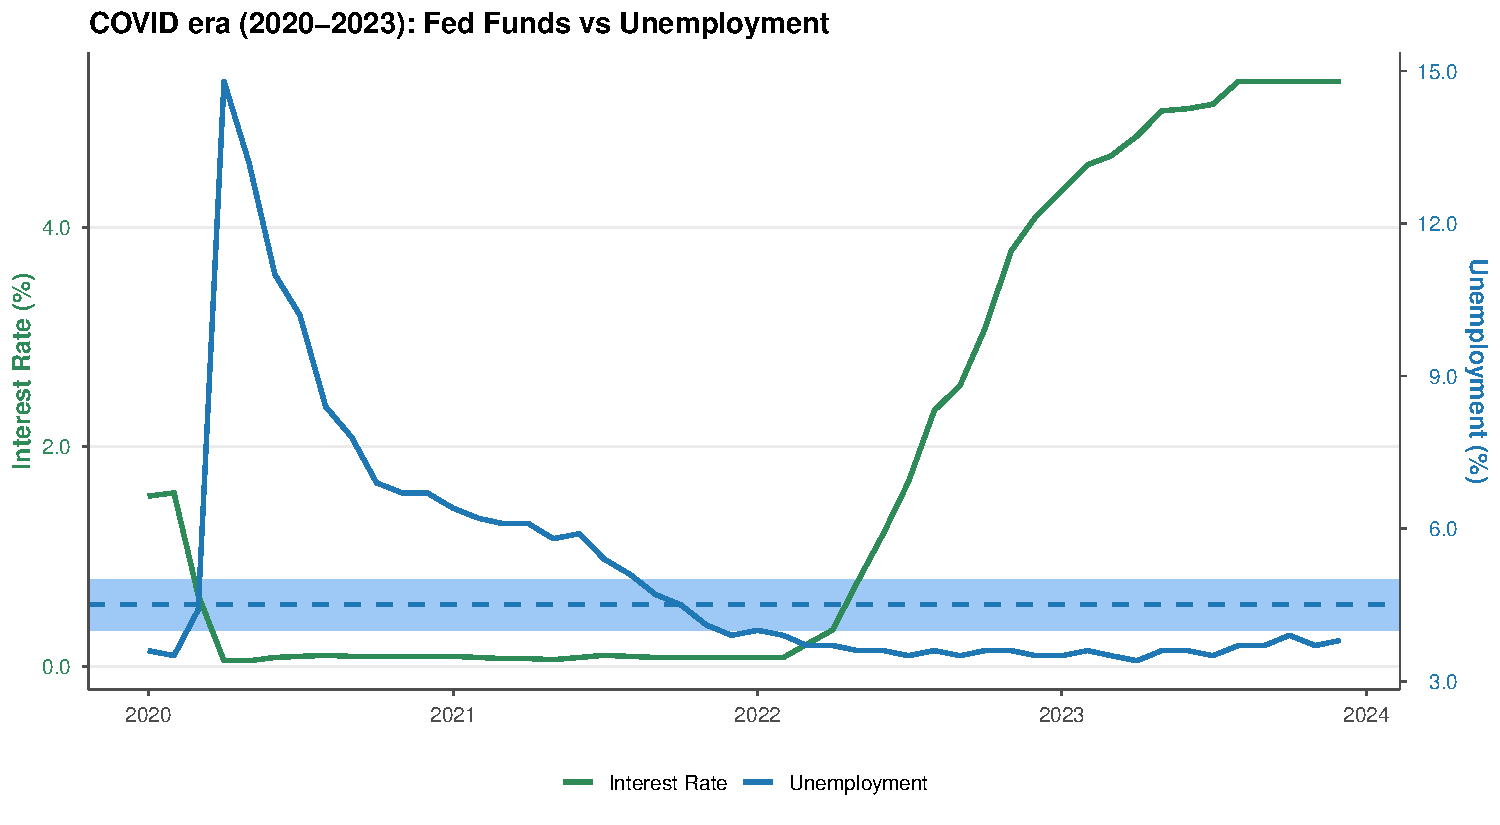
\includegraphics[keepaspectratio]{Story2_updated_files/figure-latex/51_covid_unemp-1.pdf}}

\pandocbounded{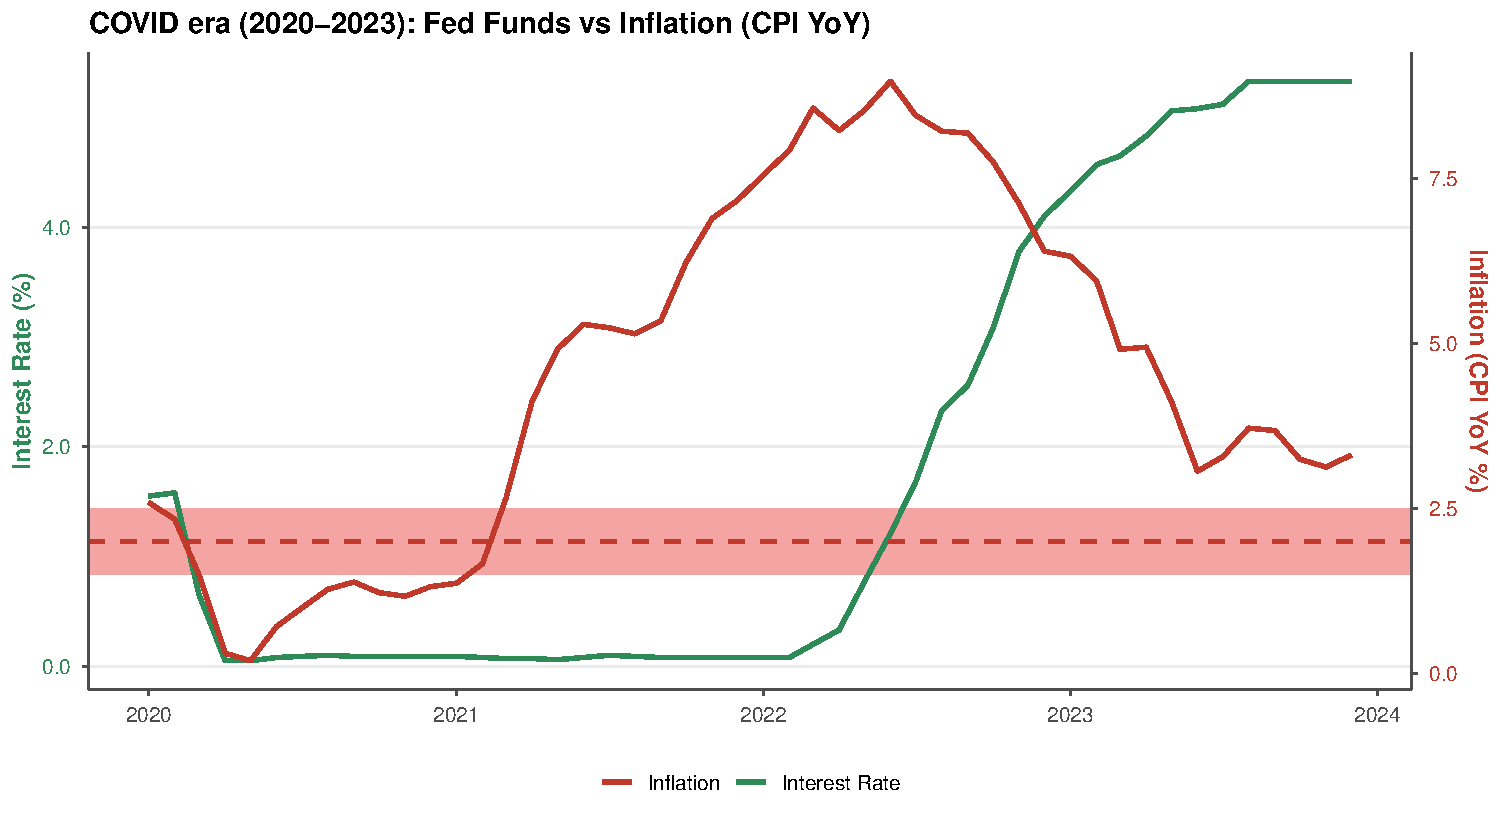
\includegraphics[keepaspectratio]{Story2_updated_files/figure-latex/52_covid_infl-1.pdf}}

\pandocbounded{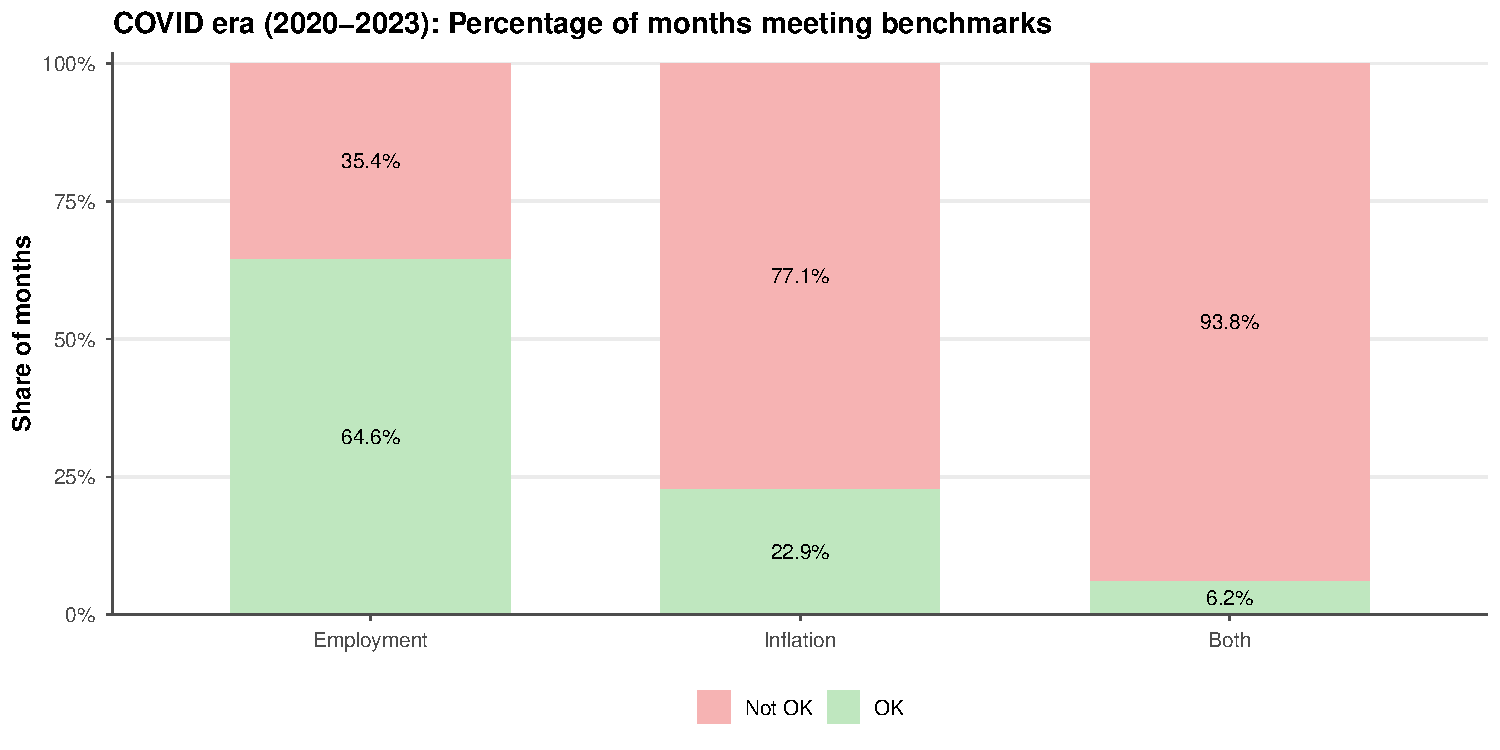
\includegraphics[keepaspectratio]{Story2_updated_files/figure-latex/52b_covid_stacked-1.pdf}}

\section{Mandate Scorecard (Quantitative
Answer)}\label{mandate-scorecard-quantitative-answer}

We use a simple benchmark definition for ``meeting both objectives'':

\begin{itemize}
\tightlist
\item
  Inflation near target: \texttt{1\%\ to\ 3\%} CPI YoY (2\% +/- 1pp
  band)\\
\item
  Labor market strong: unemployment \texttt{\textless{}=\ 5\%}
\end{itemize}

\begin{longtable}[]{@{}
  >{\raggedleft\arraybackslash}p{(\linewidth - 12\tabcolsep) * \real{0.1354}}
  >{\raggedleft\arraybackslash}p{(\linewidth - 12\tabcolsep) * \real{0.1562}}
  >{\raggedleft\arraybackslash}p{(\linewidth - 12\tabcolsep) * \real{0.1250}}
  >{\raggedleft\arraybackslash}p{(\linewidth - 12\tabcolsep) * \real{0.1562}}
  >{\raggedleft\arraybackslash}p{(\linewidth - 12\tabcolsep) * \real{0.1250}}
  >{\raggedleft\arraybackslash}p{(\linewidth - 12\tabcolsep) * \real{0.1667}}
  >{\raggedleft\arraybackslash}p{(\linewidth - 12\tabcolsep) * \real{0.1354}}@{}}
\caption{25-year mandate scorecard (monthly
observations)}\tabularnewline
\toprule\noalign{}
\begin{minipage}[b]{\linewidth}\raggedleft
months\_total
\end{minipage} & \begin{minipage}[b]{\linewidth}\raggedleft
months\_dual\_ok
\end{minipage} & \begin{minipage}[b]{\linewidth}\raggedleft
pct\_dual\_ok
\end{minipage} & \begin{minipage}[b]{\linewidth}\raggedleft
months\_infl\_ok
\end{minipage} & \begin{minipage}[b]{\linewidth}\raggedleft
pct\_infl\_ok
\end{minipage} & \begin{minipage}[b]{\linewidth}\raggedleft
months\_unemp\_ok
\end{minipage} & \begin{minipage}[b]{\linewidth}\raggedleft
pct\_unemp\_ok
\end{minipage} \\
\midrule\noalign{}
\endfirsthead
\toprule\noalign{}
\begin{minipage}[b]{\linewidth}\raggedleft
months\_total
\end{minipage} & \begin{minipage}[b]{\linewidth}\raggedleft
months\_dual\_ok
\end{minipage} & \begin{minipage}[b]{\linewidth}\raggedleft
pct\_dual\_ok
\end{minipage} & \begin{minipage}[b]{\linewidth}\raggedleft
months\_infl\_ok
\end{minipage} & \begin{minipage}[b]{\linewidth}\raggedleft
pct\_infl\_ok
\end{minipage} & \begin{minipage}[b]{\linewidth}\raggedleft
months\_unemp\_ok
\end{minipage} & \begin{minipage}[b]{\linewidth}\raggedleft
pct\_unemp\_ok
\end{minipage} \\
\midrule\noalign{}
\endhead
\bottomrule\noalign{}
\endlastfoot
299 & 83 & 27.8 & 178 & 59.5 & 147 & 49.2 \\
\end{longtable}

\begin{longtable}[]{@{}
  >{\raggedright\arraybackslash}p{(\linewidth - 14\tabcolsep) * \real{0.2993}}
  >{\raggedleft\arraybackslash}p{(\linewidth - 14\tabcolsep) * \real{0.0949}}
  >{\raggedleft\arraybackslash}p{(\linewidth - 14\tabcolsep) * \real{0.1095}}
  >{\raggedleft\arraybackslash}p{(\linewidth - 14\tabcolsep) * \real{0.0876}}
  >{\raggedleft\arraybackslash}p{(\linewidth - 14\tabcolsep) * \real{0.1095}}
  >{\raggedleft\arraybackslash}p{(\linewidth - 14\tabcolsep) * \real{0.0876}}
  >{\raggedleft\arraybackslash}p{(\linewidth - 14\tabcolsep) * \real{0.1168}}
  >{\raggedleft\arraybackslash}p{(\linewidth - 14\tabcolsep) * \real{0.0949}}@{}}
\caption{Mandate scorecard by period (monthly
observations)}\tabularnewline
\toprule\noalign{}
\begin{minipage}[b]{\linewidth}\raggedright
period
\end{minipage} & \begin{minipage}[b]{\linewidth}\raggedleft
months\_total
\end{minipage} & \begin{minipage}[b]{\linewidth}\raggedleft
months\_dual\_ok
\end{minipage} & \begin{minipage}[b]{\linewidth}\raggedleft
pct\_dual\_ok
\end{minipage} & \begin{minipage}[b]{\linewidth}\raggedleft
months\_infl\_ok
\end{minipage} & \begin{minipage}[b]{\linewidth}\raggedleft
pct\_infl\_ok
\end{minipage} & \begin{minipage}[b]{\linewidth}\raggedleft
months\_unemp\_ok
\end{minipage} & \begin{minipage}[b]{\linewidth}\raggedleft
pct\_unemp\_ok
\end{minipage} \\
\midrule\noalign{}
\endfirsthead
\toprule\noalign{}
\begin{minipage}[b]{\linewidth}\raggedright
period
\end{minipage} & \begin{minipage}[b]{\linewidth}\raggedleft
months\_total
\end{minipage} & \begin{minipage}[b]{\linewidth}\raggedleft
months\_dual\_ok
\end{minipage} & \begin{minipage}[b]{\linewidth}\raggedleft
pct\_dual\_ok
\end{minipage} & \begin{minipage}[b]{\linewidth}\raggedleft
months\_infl\_ok
\end{minipage} & \begin{minipage}[b]{\linewidth}\raggedleft
pct\_infl\_ok
\end{minipage} & \begin{minipage}[b]{\linewidth}\raggedleft
months\_unemp\_ok
\end{minipage} & \begin{minipage}[b]{\linewidth}\raggedleft
pct\_unemp\_ok
\end{minipage} \\
\midrule\noalign{}
\endhead
\bottomrule\noalign{}
\endlastfoot
Dot-com bust (2000-2003) & 35 & 4 & 11.4 & 29 & 82.9 & 8 & 22.9 \\
Financial crisis + aftermath (2008-2012) & 60 & 0 & 0.0 & 29 & 48.3 & 3
& 5.0 \\
COVID era (2020-2023) & 48 & 3 & 6.2 & 11 & 22.9 & 31 & 64.6 \\
\end{longtable}

\section{Visualization 2 --- Tradeoff Map (Inflation vs
Unemployment)}\label{visualization-2-tradeoff-map-inflation-vs-unemployment}

This ``quadrant'' view highlights when the U.S. was closest to the dual
mandate (bottom-left).

\pandocbounded{
\includegraphics[keepaspectratio]{Story2_updated_files/figure-latex/viz_scatter-1.pdf}}

\section{Conclusion: Has the Fed Fulfilled the
Mandate?}\label{conclusion-has-the-fed-fulfilled-the-mandate}

\textbf{Short answer:} \textbf{Partially, but not consistently.}

\begin{itemize}
\tightlist
\item
  The timeline and scatter show extended periods where one objective was
  met while the other was missed.\\
\item
  The strongest dual-mandate performance appears in the late-2010s
  expansion.\\
\item
  Major misses occurred in the Great Recession and pandemic labor shock
  (employment miss) and in 2021-2023 (inflation miss).
\end{itemize}

Overall, over the full 25-year window, the Fed appears able to
\textbf{restore} the mandate after shocks, but not to keep both goals
satisfied continuously.

\section{Key Takeaways (Draft Slide
Text)}\label{key-takeaways-draft-slide-text}

Use these as the narration overlay for your Manim slides:

\begin{itemize}
\tightlist
\item
  \textbf{Best ``dual mandate'' stretch:} the late 2010s, when
  unemployment was low and inflation was not persistently elevated.\\
\item
  \textbf{Employment misses:} recessions and shocks (2008--2010; 2020)
  when unemployment spikes regardless of inflation levels.\\
\item
  \textbf{Inflation miss:} 2021--2023 surge (inflation far above a 2\%
  benchmark while unemployment stayed low).\\
\item
  \textbf{Timing matters:} the Fed reacts to inflation data;
  unemployment tends to move with a lag after costs/financing tighten.
\end{itemize}

\section{Export Plots for Manim}\label{export-plots-for-manim}

\section{Next Step: Manim Animation Plan
(Outline)}\label{next-step-manim-animation-plan-outline}

\begin{enumerate}
\def\labelenumi{\arabic{enumi}.}
\tightlist
\item
  Title slide: question + dual mandate definition\\
\item
  Timeline slide: fade in panels (inflation → unemployment → fed funds)
  + episode callouts\\
\item
  Tradeoff slide: animate pointer into ``good quadrant'' and compare
  eras\\
\item
  Lag slide: annotate right-lower quadrant as ``hike → future inflation
  falls''\\
\item
  Summary slide: mandate scorecard + caveat about lags/supply shocks
\end{enumerate}

\end{document}
